\documentclass[a4paper, 11pt]{article}
\usepackage[polish]{babel}
\usepackage[T1]{fontenc}
\usepackage{hyperref}
\usepackage{array}
\usepackage{amssymb}
\hypersetup{
    colorlinks,
    citecolor=black,
    filecolor=black,
    linkcolor=black,
    urlcolor=black
}
\usepackage{graphicx}

\usepackage{tikz}
\usetikzlibrary{fit,arrows,matrix,positioning, calc, shapes.gates.logic.IEC, shapes.gates.logic.US}
\tikzstyle{branch}=[fill,shape=circle,minimum size=3pt,inner sep=0pt]


\title{%
	%\vspace{-3.5cm}
       \large Sprawozdanie Laboratorium Mikroelektronika \\
       \huge  Podstawowe symulacje wybranych układów CMOS – tranzystor nMOS}

\author{Stanisław Fiedler 160250 L1}
\date{LAB 2, 22 października 2024}

\begin{document}

\maketitle
\tableofcontents

\section{Zadanie 1}\label{sec:zadanie_1} % (fold)

\subsection{Na otrzymanych wynikach symulacji zaznaczyć obszary liniowy oraz nasycenia tranzystora
	nMOS.}\label{sub:11} % (fold)
\begin{center}
	\begin{tikzpicture}
		\node (img) {
			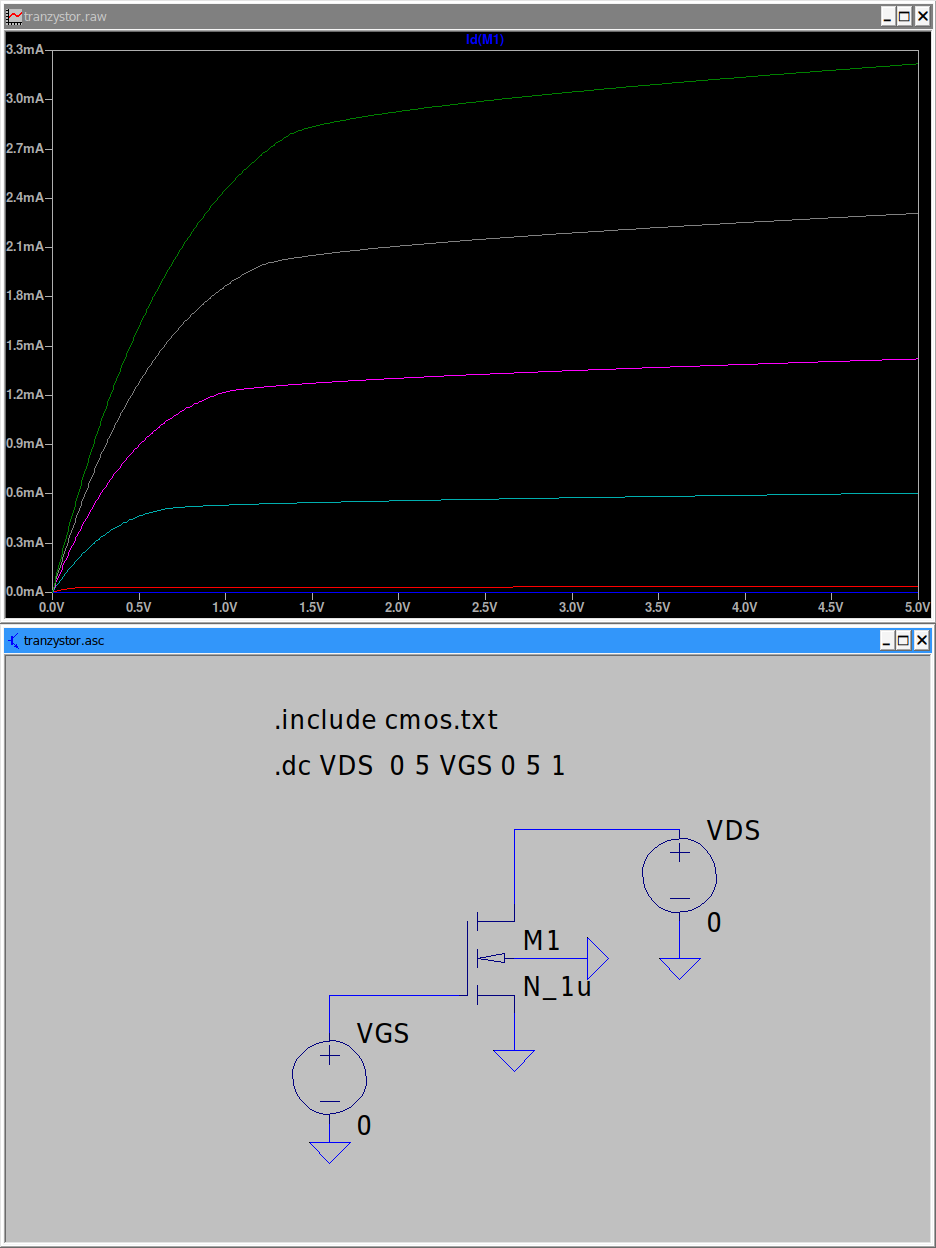
\includegraphics[scale=0.3]{images/simulation.png}
		};
		\draw[white] (-3.5,5.5) node {\large liniowy};
		\draw[white] (1,5.5) node {\large nasycenia};
		\draw[white, thick, dashed] (-4.36,0.34) .. controls (-2.75,1) and (-2,2) .. (-1.2,6);
	\end{tikzpicture}
\end{center}
% subsection  (end)

\subsection{W oparciu o wiedzę z podstaw elektroniki podać i omówić stosowne wzory wyjaśniające zasadę
	działania tranzystora nMOS.}\label{sub:12} % (fold)
Wzory opisujące działanie tranzystora nMOS:
\begin{enumerate}
	\item w zakresie odcięcia:
	      \[
		      I_D = 0
	      \]
	\item w zakresie linowym: \[
		      I_D = \mu C_{OX} \frac{W}{L} \left[ \left( V_{GS} - V_{T} \right) - \frac{V^2_{DS}}{2} \right] 	      \]
	\item w zakresie nasycenia: \[
		      I_D = \mu C_{OX} \frac{W}{L} \frac{\left( V_{GS} - V_{T} \right)^2}{2}
	      \]
\end{enumerate}
% subsection  (end)

Kiedy $ V_{DS} < V_{GS}-V_{T} $ tranzystor znajduje się w obszarze liniowym, prąd drenu zależy wtedy od napięcia $ V_{DS} $.
W zakresie tym napięcie dren-źródło nie ma większego wpływu na kanał przewodzący.

W zakresie nasycenia $ \left( V_{DS} > V_{GS}-V_{T} \right) $ z powodu działania pola elektrycznego między źródłem, a drenem, kanał przewodzący zwęża się co powoduje że $ I_D $ przestaje być zależne od napięcia dren-źródło.
Aby zwiększyć prąd drenu w zakresie nasycenia należy poszerzyć kanał zwiększając napięcie bramki.

% section Zadanie 1 (end)

\section{Co zawiera plik cmos.txt ? Jaką funkcję pełni ten plik podczas symulacji?}\label{sec:zadanie_2} % (fold)

Plik cmos.txt zawiera wartości wszystkich stałych opisujących właściwości tranzystora.
Pozwala on na przeprowadzenie symulacji zgodnej z rzeczywistym zachowaniem tranzystora.

% section Zadanie 2 (end)

\section{Co oznacza ostatnia liczba w zapisie:}\label{sec:zadanie_3} % (fold)
\begin{verbatim}
	 .model N_50n nmos level = 54 oraz .MODEL P_1u PMOS LEVEL = 3
\end{verbatim}

Ostatnia liczba oznacza poziom złożoności i dokładności z jaką jest opisany tranzystor.

% section Zadanie 3 (end)

\section{Co oznaczają w pliku bibliotecznym BSIM cmos.txt parametry VT0 oraz TOX ?}\label{sec:zadanie_4} % (fold)

\begin{description}
	\item[VT0] opisuje napięcie progowe tranzystora.
	\item[TOX] jest grubością warstwy dwutlenku krzemu $SiO_2$.
\end{description}

% section Zadanie 4 (end)

\end{document}

